% This is samplepaper.tex, a sample chapter demonstrating the
% LLNCS macro package for Springer Computer Science proceedings;
% Version 2.20 of 2017/10/04
%
\documentclass[runningheads]{llncs}
%

\usepackage{graphicx}
% Used for displaying a sample figure. If possible, figure files should
% be included in EPS format.
%
% If you use the hyperref package, please uncomment the following line
% to display URLs in blue roman font according to Springer's eBook style:
% \renewcommand\UrlFont{\color{blue}\rmfamily}


\usepackage{alltt}
%\usepackage{pslatex}
%\usepackage{epigraph}
%\usepackage{verbatim}
\usepackage{latexsym}
\usepackage{array}
\usepackage{comment}
%\usepackage{makeidx}
%\usepackage{indentfirst}
%\usepackage{verbatim}
%\usepackage{color}
%\usepackage{url}
%\usepackage{xspace}
%\usepackage{hyperref}
%\usepackage{stmaryrd}
\usepackage{amsmath}
\usepackage{amssymb}  % mathcal
%\usepackage{graphicx}
%\usepackage{euscript}
\usepackage{mathtools}
%\usepackage{mathrsfs}
%\usepackage{multirow,bigdelim}
%\usepackage{subcaption}
%\usepackage{placeins}
\usepackage{csvsimple}
\usepackage{array}

%\usepackage{geometry}
%\geometry{
%     top=25pt, bottom=14pt, inner=21pt, outer=21pt,
%     paperwidth=5.5in, paperheight=8.5in,
%     }
\usepackage{color}



%% Some recommended packages.
\usepackage{booktabs}   %% For formal tables:
                        %% http://ctan.org/pkg/booktabs
\usepackage{subcaption} %% For complex figures with subfigures/subcaptions
                        %% http://ctan.org/pkg/subcaption
\captionsetup{compatibility=false}

\usepackage{multirow}

\usepackage{placeins}

\usepackage{lmodern}

\usepackage{listings}
\lstdefinelanguage{ocanren}{
keywords={run, conde, fresh, let, in, match, with, when, class, type,
object, method, of, rec, repeat, until, while, not, do, done, as, val, inherit,
new, module, sig, deriving, datatype, struct, if, then, else, open, private, virtual, include, success, failure, switch, 
true, false},
sensitive=true,
commentstyle=\small\itshape\ttfamily,
keywordstyle=\ttfamily\textbf,
identifierstyle=\ttfamily,
basewidth={0.5em,0.5em},
columns=fixed,
mathescape=true,
fontadjust=true,
literate={fun}{{$\lambda$}}1 {->}{{$\to$}}3 {===}{{$\equiv$}}1 {=/=}{{$\not\equiv$}}1 {|>}{{$\triangleright$}}3 {\\/}{{$\vee$}}2 {/\\}{{$\wedge$}}2 {^}{{$\uparrow$}}1 
%{[]}{{\texttt|[]|}}1
,
morecomment=[s]{(*}{*)}
}

\lstset{
%mathescape=true,
%basicstyle=\small,
%identifierstyle=\ttfamily,
%keywordstyle=\bfseries,
%commentstyle=\scriptsize\rmfamily,
%basewidth={0.5em,0.5em},
%fontadjust=true,
language=ocanren
}

\newcommand{\lstquot}[1]{``\lstinline{#1}''}
\newcommand{\sembr}[1]{\llbracket{#1}\rrbracket}
\newcommand\false{$f\!alse$}
\newcommand\myif{i\!f}


\def\transarrow{\xrightarrow}
\newcommand{\setarrow}[1]{\def\transarrow{#1}}

\def\padding{\phantom{X}}
\newcommand{\setpadding}[1]{\def\padding{#1}} 

\def\subarrow{}
\newcommand{\setsubarrow}[1]{\def\subarrow{#1}}

\newcommand{\trule}[2]{\dfrac{#1}{#2}}
\newcommand{\crule}[3]{\dfrac{#1}{#2},\;{#3}}
\newcommand{\withenv}[2]{{#1}\vdash{#2}}
\newcommand{\trans}[3]{{#1}\transarrow{\padding{\textstyle #2}\padding}\subarrow{#3}}
\newcommand{\ctrans}[4]{{#1}\transarrow{\padding#2\padding}\subarrow{#3},\;{#4}}
\newcommand{\llang}[1]{\mbox{\lstinline[mathescape]|#1|}}
\newcommand{\pair}[2]{\inbr{{#1}\mid{#2}}}
\newcommand{\inbr}[1]{\left<{#1}\right>}
\newcommand{\highlight}[1]{\color{red}{#1}}
%\newcommand{\ruleno}[1]{\eqno[\scriptsize\textsc{#1}]}
\newcommand{\ruleno}[1]{\mbox{[\textsc{#1}]}}
\newcommand{\rulename}[1]{\textsc{#1}}
\newcommand{\inmath}[1]{\mbox{$#1$}}
\newcommand{\lfp}[1]{fix_{#1}}
\newcommand{\gfp}[1]{Fix_{#1}}
\newcommand{\vsep}{\vspace{-2mm}}
\newcommand{\supp}[1]{\scriptsize{#1}}
\renewcommand{\sembr}[1]{\llbracket{#1}\rrbracket}
\newcommand{\cd}[1]{\texttt{#1}}
\newcommand{\free}[1]{\boxed{#1}}
\newcommand{\binds}{\;\mapsto\;}
\newcommand{\dbi}[1]{\mbox{\bf{#1}}}
\newcommand{\sv}[1]{\mbox{\textbf{#1}}}
\newcommand{\bnd}[2]{{#1}\mkern-9mu\binds\mkern-9mu{#2}}
\newcommand{\meta}[1]{{\mathcal{#1}}}
\newcommand{\dom}[1]{\mathtt{dom}\;{#1}}
%\newcommand{\primi}[2]{\mathbf{#1}\;{#2}}
\renewcommand{\dom}[1]{\mathcal{D}om\,({#1})}
\newcommand{\ran}[1]{\mathcal{VR}an\,({#1})}
\newcommand{\fv}[1]{\mathcal{FV}\,({#1})}
\newcommand{\tr}[1]{\mathcal{T}r_{#1}}
\newcommand{\diseq}{\not\equiv}
\newcommand{\reprfunset}{\mathcal{R}}
\newcommand{\reprfun}{\mathfrak{f}}
\newcommand{\cstore}{\Omega}
\newcommand{\cstoreinit}{\cstore_\epsilon^{init}}
\newcommand{\csadd}[3]{add(#1, #2 \diseq #3)}  %{#1 + [#2 \diseq #3]}
\newcommand{\csupdate}[2]{update(#1, #2)}  %{#1 \cdot #2}
\newcommand{\primi}[1]{\mathbf{#1}}
\newcommand{\sem}[1]{\llbracket #1 \rrbracket}
\newcommand{\ir}{\ensuremath{\mathcal{S}}}
\usepackage{tikz}
\newcommand*\circled[1]{\tikz[baseline=(char.base)]{
    \node[shape=circle,draw,inner sep=1pt] (char) {#1};}}

\let\emptyset\varnothing
\let\eps\varepsilon

\newtheorem{Observation}{Observation}

\usepackage{float}

\begin{document}
%
\title{Relational Synthesis for Pattern Matching\thanks{This work was partially supported by the grant 18-01-00380 from The Russian Foundation for Basic Research.\\
\textcolor{red}{TODO: Get right orchid ID!}}}
%
%\titlerunning{Abbreviated paper title}
% If the paper title is too long for the running head, you can set
% an abbreviated paper title here
%
\author{Dmitry Kosarev\inst{1,2,3}\orcidID{0000-0002-6773-5322} \and
Dmitry Boulytchev\inst{1,2,4}\orcidID{6666-6666-6666-6666}
}
%
\authorrunning{D. Kosarev \& D.  Boulytchev}
% First names are abbreviated in the running head.
% If there are more than two authors, 'et al.' is used.
%
\institute{Saint Petersburg State University, Russia \and
JetBrains Research, Russia\and 
\email{Dmitrii.Kosarev@pm.me}\and 
\email{dboulytchev@math.spbu.ru}
}
%
\maketitle              % typeset the header of the contribution
%
\begin{abstract}
   We apply relational programming techniques to the problem of synthesizing efficient implementation for a pattern matching construct. Although in principle
   pattern matching can be implemented in a trivial way, the result suffers from inefficiency in terms of both performance and code size. Thus, in implementing functional languages alternative, more elaborate  approaches are widely used. However, as there are multiple kinds and flavors of pattern
   matching constructs, these approaches have to be specifically developed and justified for each concrete inhabitant of the pattern matching ``zoo.'' We formulate the
   pattern matching synthesis problem in relational terms and develop optimizations which improve the efficiency of the synthesis and guarantee the
   optimality of the result. Our approach is based on relational representations of both the high-level semantics of pattern matching and the semantics of
   an intermediate-level implementation language. This choice make our approach, in principle, more scalable as we only need to modify the high-level semantics in order
   to synthesize the implementation of a new feature. Our evaluation on a set of small samples, partially taken from existing literature shows, that our framework is
   capable of synthesizing optimal implementations quickly. Our in-depth stress evaluation on a number of artificial benchmarks, however,
   has shown the need for future improvements.

\keywords{relational programming \and relational interpreters \and pattern matching.}
\end{abstract}

\section{Introduction}
\label{sec:intro}

Algebraic data types (ADT) is an important tool in functional programming which delivers a way to represent flexible and easy to manipulate data structures.
To inspect the contents of ADT values a generic construct~--- \emph{pattern matching}~--- is used. Pattern matching can be considered as a generalization of
conventional conditional control-flow construct ``\lstinline|if .. then .. else|'' and in principle can be decomposed into a nested hierarchy of those; from
this standpoint the problem of pattern matching implementation can be considered trivial. However, some decompositions are obviously better than others. We
repeat here an example from~\cite{maranget2008} to demonstrate this difference (see Fig.~\ref{fig:match-example}). Here we match a triple of boolean
values $x$, $y$, and $z$ against four pattern (Fig.~\ref{fig:matching-example1}; we use \textsc{OCaml}~\cite{ocaml} as reference language). The na\"{i}ve
implementation of this example is shown on Fig.~\ref{fig:matching-example2}; however if we decide to match $y$ first the result becomes much
better (Fig.~\ref{fig:matching-example3}).

\begin{figure}[ht]
\begin{subfigure}[t]{0.2\linewidth}
\centering
\begin{lstlisting}
match x, y, z with
| _, F, T -> 1
| F, T, _ -> 2
| _, _, F -> 3
| _, _, T -> 4
\end{lstlisting}
\vskip18.5mm
\caption{Pattern matching}
\label{fig:matching-example1}
\end{subfigure}
\hspace{0.5cm}
\begin{subfigure}[t]{0.26\linewidth}
\centering
\begin{lstlisting}
if x then
  if y then
    if z then 4 else 3
  else
    if z then 1 else 3
else
  if y then 2
  else
    if z then 1 else 3
\end{lstlisting}
\caption{A correct but non-optimal\\\phantom{(b)~}implementation}
\label{fig:matching-example2}
\end{subfigure}
\hspace{0.5cm}
\begin{subfigure}[t]{0.33\linewidth}
\centering
\begin{lstlisting}
if y then
  if x then
    if z then 4 else 3
  else 2
else
  if z then 1 else 3
\end{lstlisting}
\vskip13.5mm
\caption{Optimal implementation}
\label{fig:matching-example3}
\end{subfigure}
\caption{Pattern matching implementation example} 
\label{fig:match-example}
\end{figure}

\begin{comment}
\begin{figure}[ht]
\begin{minipage}[b]{0.3\linewidth}
\centering
\label{fig:figure1}
\end{minipage}
\hspace{0.5cm}
\begin{minipage}[b]{0.3\linewidth}
\centering
\begin{lstlisting}
switch x with 
| true -> 
    switch y with 
    | true -> 
       switch z with 
       | true -> 4
       | _ -> 3
    | _ -> 
      switch z with 
      | true -> 1
      | _ -> 3 
| _ -> 
   switch y with 
   | true -> 2 
   | _ -> if z then 1 else 3
\end{lstlisting}
\end{minipage}
\hspace{0.5cm}
\begin{minipage}[b]{0.3\linewidth}
\centering
\end{minipage}
\end{figure}
\end{comment}


%clasification 1
Although semantics of pattern matching can be given as a sequence of srutinee's sub expression comparisons (Figure~\ref{fig:matchpatts}) effective compilers don't follow
this approach. One can either optimise runtime cost by minimizing amount of checks performed or static cost by minimizing the size of generated code. \emph{Decision trees}~\cite{?}
are good for the first criteria, because they check every subexpression not more than once. \emph{Backtracking automata} are rather compact but in some cases can perform
repeated checks.

%clasification 2
\emph{For strict languages} checking sub-expressions of scrutinee in any order is allowed. \emph{For lazy languages} pattern matching should evaluate only those sub-expressions which are
necessary for performing pattern matching. If not careful pattern matching can change the termination behavior of the program. In general lazy languages setup more constraints on pattern matching and because of that allow lesser set of heuristics. Decision trees and backtracking automata can be used for compilation both  strict and lazy languages.

%clasification 3
The matching compilers for strict languages can work in \emph{direct} or \emph{indirect} styles. The first ones return efficient code immediately. In the second style to
construct final answer some post processing is required. It can vary from easy simplifications to complicated supercompilation techniques~\cite{sestoft1996}. The main
drawback of indirect style is that the size of intermediate data structures can be exponentially large.

% about lazy languages
A few approaches for checking sub-expressions in lazy languages has been proposed. In ~\cite{augustsson1985} simple left-to-right order of subexpression checking was proposed and was proved that it doesn't affect termination. The backtracking automaton being built has a form of a DAG to reduce code size. A few refinements has been added by~\cite{wadler1987} as a part of textbook~\cite{peytonjones1987} about implementing lazy functional languages. The implementation from this book is being used in the current version of GHC~\cite{ghc}. \cite{laville1991} models values in lazy languages
using \emph{partial terms}, although it doesn't scale to types with infinite constructor sets (like integers). The approach doesn't test all subexpressions from left to right as~\cite{augustsson1985} but aims to not perform unnecessary check by constructing \emph{lazy automaton}. 
%In~\cite{suarez1993} the similar approach is extended by special treatment of overlapping patterns.

% about decision trees
Pattern matching for lazy languages has been compiled also to decision trees~\cite{maranget1992} and later (\cite{maranget1994}) into
\emph{decision DAGs} which allow in some cases to make code smaller.

Minimizing the size of decision tree is known to be NP-hard~\cite{baudinet1985tree}, and as a rule various heuristics are applied during compilation, for example, the number of nodes,
the length of the longest path, the average length of all paths. The paper~\cite{Scott2000WhenDM} performs experimental evaluation of nine heuristics on the base of for strict language Standard ML of New Jersey.

%about automata
The inefficiency of backtracking automaton has been
improved in~\cite{maranget2001}. The approach utilizes matrix representation for pattern matching. It splits the current matrix according to constructors in the
first column and reduces the task to compiling matrices with less rows. The technique is indirect, in the end a few optimizations are performed by introducing
special \emph{exit} nodes to the compiled representation. No preprocessing is required for this scheme: or-pattern receives a special treatment during compilation process.
The approach from this paper is used in the current implementation of the \textsc{OCaml} compiler.

Previous approach uses first column to split the matrix. In~\cite{maranget2008} the \emph{necessity} heuristic has been introduced which recommends which column should be
used to perform the split. Good decision trees which are constructed in this work can perform better on corner cases than~\cite{maranget2001}, but for practical cases the
difference is insignificant.


While existing approaches deliver appropriate solutions for certain forms of pattern matching construct, they have to be extended in an \emph{ad hoc} manner each time
the syntax and semantics of pattern matching construct changes. For example, besides a simple conventional form of pattern matching there is a number of extensions
(guards~\cite{?}, disjunctive patterns~\cite{?}, non-linear patterns~\cite{mcbride1969symbol}, active patterns~\cite{activepatterns}, pattern matching for polymorphic variants~\cite{Garrigue98} and generalized
algebraic datatypes~\cite{?}) which require a separate customized algorithms to be developed.

\begin{comment}
\begin{minipage}[b]{0.5\textwidth}
There are a few different approaches for compiling pattern mathcing. For example, \textsc{GHC}~\cite{?} uses that presented in an influential paper~\cite{Jones1987},
implementation of pattern matching in \textsc{OCaml} is currently based on~\cite{maranget2001} although \cite{maranget2008} reports a slight improvements
of generated code efficiency. 
\end{minipage}
\end{comment}

We present an approach to pattern matching implementation based on application of relational programming~\cite{TRS,WillThesis} and, in particular, relational interpreters~\cite{unified}
and relational conversion~\cite{lozov2017}. Our approach is based on relational representation of the top-level source language semantics of pattern matching on the one hand, and
the semantics of intermediate-level implementation language on the other. We formulate the condition for a correct and complete implementation of pattern matching and use it to
construct a top-level goal which represents a search procedure for all correct and complete implementations. We also present a number of techniques which makes it possible to come up with an
\emph{optimal} solution as well as optimizations to improve the performance of the search. Our implementation\footnote{\url{https://github.com/kakadu/pat-match}} makes use of
\textsc{OCanren}\footnote{\url{https://github.com/JetBrains-Research/OCanren}}~--- a typed implementation of \textsc{miniKanren} for \textsc{OCaml}~\cite{OCanren},
and \textsc{noCanren}\footnote{\url{https://github.com/Lozov-Petr/noCanren}}~--- a convertor from the subset of plain \textsc{OCaml} into \textsc{OCanren}~\cite{lozov2017}.
An evaluation, performed for a set of benchmarks taken from other papers, initially has shown a good performance of our synthesizer. However, being aware of some pitfalls of
our approach, we came up with a set of counterexamples, on which it did not provide any results in observable time, so we do not consider the problem completely solved.
We also started a work on mechanized formalization\footnote{\url{https://github.com/dboulytchev/Coq-matching-workout}}, written in \textsc{Coq}~\cite{Coq}, to
make the justification of out approach more solid and easier to verify, but this formalization is not yet complete. 

 

\section{The Pattern Matching Synthesis Problem}

We describe here a simplified view on pattern matching which does not incorporate some practically important aspects of the construct such as
name bindings in patterns, guards or even semantic actions in branches. In a purified form, however, it  represents the essence of pattern
matching as an ``inspect-and-branch'' procedure. Other features can be easily added later once a solution for the essential part of the problem
is found.

First, we introduce a finite set of \emph{constructors} $\mathcal C$, equipped with arities, a set of values $\mathcal{V}$
and a set of patterns $\mathcal{P}$:
 
\[
 \begin{array}{rcll}
    \mathcal{C} & = & \{ C_1^{k_1}, \dots, C_n^{k_n} \}\\
    \mathcal{V} & = & \mathcal{C}\,\mathcal{V}^*\\  
    \mathcal{P} & = & \_ \mid \mathcal{C}\,\mathcal{P}^*
 \end{array}
\]

We define a matching of a value $v$ (\emph{scrutinee}) against an ordered non-empty sequence of patterns $p_1,\dots,p_k$ by means of the following
relation

\[
\setarrow{\xrightarrow}
\trans{\inbr{v;\,p_1,\dots,p_k}}{}{i},\,1\le i\le k+1
\]

which gives us the index of the leftmost matched pattern or $k+1$ if no such pattern exists. We use an auxiliary relation $\inbr{;}\subseteq\mathcal{V}\times\mathcal{P}$
to specify the notion of a value matched by an individual pattern (see Fig.~\ref{fig:match1pat}). The rule \ruleno{Wildcard} says that
a wildcard pattern ``\_'' matches any value, and \ruleno{Constructor} specifies that a constructor pattern matches exactly those values which
have the same constructor at the top level and all subvalues matched by corresponding subpatterns. The definition of ``$\xrightarrow{}{\!\!}$'' is
shown on Fig.~\ref{fig:matchpatts}. An auxiliary relation
 ``$\xrightarrow{}{}_{\!\!*}$'' 
is introduced to specify the left-to-right matching strategy, and we
use current index as an environment. An important rule, $\ruleno{MatchOtherwise}$ specifies that if we exhausted all the patterns with no matching we stop with
the current index (which in this case is equal to the number of patterns plus one).

\begin{figure}[t]
   \renewcommand*{\arraystretch}{2}
   \[
   \begin{array}{cr}
     \inbr{v;\,\_} & \ruleno{Wildcard} \\
     \trule{\forall i\;\inbr{v_i;\,p_i}}{\inbr{C^k\,v_1\dots v_k;\,C^k\,p_1\dots p_k}},\,k\ge 0 & \ruleno{Constructor}
   \end{array}
   \]
   \caption{Matching against a single pattern}
   \label{fig:match1pat}
\end{figure}

\begin{figure}[t]
   \renewcommand*{\arraystretch}{3}
   \setarrow{\xrightarrow}
   \setsubarrow{_*}
   \[
   \begin{array}{cr}
     \trule{\inbr{v;\,p_1}}
           {\withenv{i}{\trans{\inbr{v;\,p_1,\dots,p_k}}{}{i}}} & \ruleno{MatchHead}\\
     \trule{\neg\inbr{v;\,p_1}\qquad\withenv{i+1}{\trans{\inbr{v;\,p_2,\dots,p_k}}{}{j}}}
           {\withenv{i}{\trans{\inbr{v;\,p_1,\dots,p_k}}{}{j}}} & \ruleno{MatchTail}\\
     \withenv{i}{\trans{\inbr{v;\,\varepsilon}}{}{i}} & \ruleno{MatchOtherwise}\\
     \trule{\withenv{1}{\trans{\inbr{v;\,p_1,\dots,p_k}}{}{i}}}
           {\setsubarrow{}\trans{\inbr{v;\,p_1,\dots,p_k}}{}{i}} & \ruleno{Match}
   \end{array}
   \]
   \caption{Matching against an ordered sequence of patterns}
   \label{fig:matchpatts}
\end{figure}

The relation ``$\xrightarrow{}{}\!\!$'' gives us a \emph{declarative} semantics of pattern matching. Since we are interested in
synthesizing implementations, we need a \emph{programmatical} view on the same problem. Thus, we introduce a language $\mathcal S$
(the ``switch'' language) of test-and branch constructs:

\[
\begin{array}{rccl}
  \mathcal M & = &       & \bullet \\
             &   & \mid  & \mathcal M\,[\mathbb{N}] \\
  \ir        & = &       & \primi{return}\,\mathbb{N} \\
             &   & \mid  & \primi{switch}\;\mathcal{M}\;\primi{with}\; [\mathcal{C}\; \primi{\rightarrow}\; \ir]^*\;\primi{otherwise}\;\ir
\end{array}
\]
 
Here $\mathcal{M}$ stands for a \emph{matching expression}, which is either a reference to a scrutinee ``$\bullet$'' or
a (multiply) indexed subexpression of a scrutinee. Programs in the switch language can discriminate on the
structure of matching expressions, testing their top-level constructors and eventually returning natural numbers as results.
The switch language is similar to the intermediate representations for pattern matching code used in 
previous works on pattern matching implementation~\cite{maranget2001,maranget2008}, and switch programs are analogous to
\emph{decision trees}.

The semantics of the switch language is given by mean of relations ``$\xrightarrow{}{}_{\!\!\!\mathcal M}$'' and ``$\xrightarrow{}{}_{\!\!\mathcal S}$''
(see Fig.~\ref{fig:matchexpr} and \ref{fig:test-and-branch}). The first one describes the semantics of matching expression, while
the second describes the semantics of the switch language itself. In both cases the scrutinee $v$ is used as an environment ($v\vdash$).


\begin{figure}[t]
  \renewcommand*{\arraystretch}{2}
  \setarrow{\xrightarrow}
  \setsubarrow{_{\mathcal M}}
  \[
  \begin{array}{cr}
    \withenv{v}{\trans{\bullet}{}{v}} & \ruleno{Scrutinee} \\
    \trule{\withenv{v}{\trans{m}{}{C^k v_1\dots v_k}}}{\withenv{v}{\trans{m[i]}{}{v_i}}} & \ruleno{SubMatch} 
  \end{array}
  \]
  \caption{Semantics of matching expression}
  \label{fig:matchexpr}
\end{figure}

\begin{figure}[t]
  \setarrow{\xrightarrow}
  \setsubarrow{_{\mathcal S}}
  \[
  \begin{array}{cr}
    \withenv{v}{\trans{\primi{return}\;i}{}{i}} & \ruleno{Return}\\[10mm]
    
    \trule{\renewcommand*{\arraystretch}{1}
           \begin{array}{c}        
              {\setsubarrow{_{\mathcal M}}\withenv{v}{\trans{m}{}{C^k\ v_1 \dots v_k}}} \\
              \withenv{v}{\trans{s}{}{i}}
           \end{array}
          }    
          {\withenv{v}{\trans{\primi{switch}\;m\;\primi{with}\;[C^k\to s]s^*\;\primi{otherwise}\;s^\prime}{}{i}}} & \ruleno{SwitchMatched}\\[10mm]
          
    \trule{\renewcommand*{\arraystretch}{1}
           \begin{array}{c}        
             {\setsubarrow{_{\mathcal M}}\withenv{v}{\trans{m}{}{D^n\  v_1 \dots v_n}}}\\
             C^k\ne D^n\\
             \withenv{v}{\trans{\primi{switch}\;m\;\primi{with}\;s^*\;\primi{otherwise}\;s^\prime}{}{i}}
           \end{array}
          }
          {\withenv{v}{\trans{\primi{switch}\;m\;\primi{with}\;[C^k\to s]s^*\;\primi{otherwise}\;s^\prime}{}{i}}} & \ruleno{SwitchNotMatched}\\[10mm]
          
    \trule{\withenv{v}{\trans{s}{}{i}}}{\withenv{v}{\trans{\primi{switch}\;m\;\primi{with}\;\varepsilon\;\primi{otherwise}\;s}{}{i}}} & \ruleno{SwitchOtherwise}
  \end{array}
  \]
  \caption{Semantics of switch programs}
  \label{fig:test-and-branch}
\end{figure}

The following observations can be easily proven by structural induction.

\begin{Observation}
  For arbitrary pattern the set of matching values is non-empty:

  \[
  \forall p\in\mathcal P : \{v\in\mathcal V\mid \inbr{v;\,p}\}\ne\emptyset
  \]
\end{Observation}

\begin{Observation}
  Relations ``$\xrightarrow{}{}\!\!\!$'' and ``$\xrightarrow{}{}_{\!\!\mathcal S}$'' are functional and deterministic respectively:

  \[
  \setarrow{\xrightarrow}
  \begin{array}{rcl}
    \forall p_1,\dots,p_k\in\mathcal P,\,\forall v\in \mathcal V,\,\forall \pi\in\mathcal S & : & |\{i\in\mathbb N\mid \trans{\inbr{v;\,p_1,\dots,p_k}}{}{i}\}|=1 \\
                                                                 &  & {\setsubarrow{_{\mathcal S}}|\{i\in\mathbb N\mid \withenv{v}{\trans{\pi}{}{i}}\}|\le 1}
  \end{array}
  \]
\end{Observation}

With these definitions, we can formulate the \emph{pattern matching synthesis problem} as follows: for a given ordered sequence of patterns $p_1,\dots,p_k$ find
a switch program $\pi$, such that

\[
\setarrow{\xrightarrow}
\forall v\in \mathcal V,\; \forall 1\le i\le n+1 : \trans{\inbr{v;\,p_1,\dots,p_n}}{}{i}\Longleftrightarrow{\setsubarrow{_{\mathcal S}}\withenv{v}{\trans{\pi}{}{i}}}\eqno{(\star)}
\]

In other words, program $\pi$ delivers a correct and complete implementation for pattern matching.

\section{Pattern Matching Synthesis, Relationally}
\label{sec:relationally}

In this section we describe a relational formulation for the pattern matching synthesis problem. Practically,
this amounts to constructing a goal with a free variable corresponding to the switch program to synthesize
for (arbitrary) list of patterns. In order to come up with a tractable goal certain steps have to be performed.
We first describe the general idea, and then consider these steps is details.

Our idea of using relational programming for pattern matching synthesis is based on the following observations:

\begin{itemize}
\item For the switch language we can implement a relational interpreter\footnote{Conventionally for \textsc{miniKanren},
  the names of relations are superscripted by ``$^o$''.} $eval^o_\ir$ with the following property: for
  arbitrary $v\in\mathcal V$, $\pi\in\ir$ and $i\in\mathbb N$
 
  \[
  \setarrow{\xrightarrow}
  \setsubarrow{_\ir}
   eval^o_\ir\, v\, \pi\, i \Longleftrightarrow \withenv{v}{\trans{\pi}{}{i}}
  \]

  In other words, $eval^o_\ir$ interprets a program $\pi$ for a scrutinee $v$ and returns exactly the same branch (if any)
  which is prescribed by the semantics of the switch language. 
  
\item On the other hand, we can directly encode the declarative semantics of pattern matching as a relational
  program $match^o$ such that for arbitrary $v\in\mathcal V$, $p_i\in\mathcal P$ and $i\in\mathbb N$

  \[
  \setarrow{\xrightarrow}
  match^o\,v\,p_1,\dots,p_k\,i \Longleftrightarrow \trans{\inbr{v;\,p_1,\dots,p_k}}{}{i}
  \]

  Again, $match^o$ succeeds with $1\le i\le k$ iff $p_i$ is the leftmost pattern, matching $v$; otherwise it
  succeeds with $i=k+1$.
\end{itemize}

We address the construction of relational interpreters for both semantics in Section~\ref{sec:relints}.

Being relational, both $eval^o_\ir$ and $match^o$ do not just succeed or fail for ground arguments, but also can be \emph{queried} for
arguments with free logical variables, thus performing a search for all substitutions for these variables which make the
relation hold. This observation leads us to the idea of utilizing the definition of the pattern matching
synthesis problem, replacing ``$\xrightarrow{}{}\!\!$'' with $match^o$, ``$\xrightarrow{}{}_{\!\!\!\mathcal S}$`` with $eval^o$,
and $\pi$ with a free logical variable $\circled{?}$, which gives us the goal

\[
\forall v\in \mathcal V,\; \forall 1\le i\le n+1 : match^o\,v\,p_1,\dots,p_n\,i\Longleftrightarrow eval^o\,v\,\circled{?}\,i
\]

\noindent This goal, however, is problematic from relational point of view due to a number of reasons.

First, \textsc{miniKanren} provides rather a limited support for universal quantification. Apart from being inefficient from
a performance standpoint, existing implementations either do not coexist with disequality constraints~\cite{eigen}
or do not support quantified goals with infinite number of answers~\cite{moiseenko}. As we will see below, both restrictions are
violated in our case. Second, there is no direct support for the equivalence of goals (``$\Leftrightarrow$''). Thus,
reducing the original synthesis problem to a viable relational goal involves some ``massaging''.

We eliminate the universal quantification over the infinite set of scrutinees, replacing it by a \emph{finite}
conjunction over a \emph{complete set of samples}. For a sequence of patterns $p_1,\dots,p_k$ a
complete set of samples is a finite set of values $\mathcal{E}(p_1,\dots,p_k)\subseteq\mathcal{V}$ with the following
property:

\[
\setarrow{\xrightarrow}
\begin{array}{rcl}
  \forall\pi\in\mathcal S & : & [\forall v\in\mathcal{E}(p_1,\dots,p_k),\,\forall i\in\mathbb{N} : \trans{\inbr{v;\,p_1,\dots,p_k}}{}{i} \Longleftrightarrow {\setsubarrow{_{\mathcal S}}\withenv{v}{\trans{\pi}{}{i}}}] \Longrightarrow \\
                          &   & [\forall v\in\mathcal V,\,\forall i\in\mathbb{N} : \trans{\inbr{v;\,p_1,\dots,p_k}}{}{i} \Longleftrightarrow  {\setsubarrow{_{\mathcal S}}\withenv{v}{\trans{\pi}{}{i}}}]
\end{array}
\]

In other words, if a program implements a correct and complete pattern matching for all values in a complete set of samples, then this
program implements a correct and complete pattern matching for all values. The idea of using a complete set of samples originates from the following observation: each pattern
describes a (potentially infinite) set of values, and pattern matching splits the set of all values into equivalence classes, each corresponding to a certain matching pattern.
Moreover, the values of different classes can be distinguished only by looking down to a \emph{finite} depth (as different patterns can be distinguished in this way).
The generation of complete sample set will be addressed below (see Section~\ref{sec:samples}). Example-based program synthesis is not a completely new technique in relational
programming~\cite{unified}; in our case, however, we can ensure the correctness of the synthesis result, while in previous reports it had to be established externally.

\setarrow{\xrightarrow}

To eliminate the universal quantification over the set of answers we rely on the functionality of declarative pattern matching semantics. Indeed, given a fixed sequence $p_1,\dots,p_k$
of patterns, for every value $v$ there is exactly one answer value $i$, such that $\trans{\inbr{v;\,p_1,\dots,p_k}}{}{i}$. We can reformulate this property as

\[
\exists i:\, \trans{\inbr{v;\,p_1,\dots,p_k}}{}{i} \Longrightarrow  
\big(\forall j : \trans{\inbr{v;\,p_1,\dots,p_k}}{}{j} \Longrightarrow  j=i\large\big)
\]

Thus, we can replace universal quantification over the sets of answers by existential one, for which we have an efficient relational counterpart~--- the ``\lstinline|fresh|''
construct.

Following the same argument, we may replace the equivalence with conjunction: indeed, if

\[
\setarrow{\xrightarrow}
\trans{\inbr{v;\,p_1,\dots,p_k}}{}{i}
\]

for some $i$, then (by functionality), for any other $j\ne i$

\[
\setarrow{\xrightarrow}
\neg\;(\trans{\inbr{v;\,p_1,\dots,p_k}}{}{j})
\]

A correct pattern matching implementation $\pi$ should satisfy the condition

\[
\setarrow{\xrightarrow}
\setsubarrow{_{\mathcal S}}
\withenv{v}{\trans{\pi}{}{i}}
\]

But, by the determinism of the switch language semantics, it immediately follows, that for arbitrary $j\ne i$

\[
\setarrow{\xrightarrow}
\setsubarrow{_{\mathcal S}}
\neg\;(\withenv{v}{\trans{\pi}{}{j}})
\]

\begin{comment}
Alternatively\footnote{\color{red} Reviewer N1 said that passage about bool argument is unclear and may be omitted (or described with more details)}, we could switch to a more explicit relational representation of both semantics, adding an extra boolean argument to
both $eval^o_{\mathcal S}$ and $match^o$ and using the same fresh variable $b$ in the query of interest:

\[
match^o\,v\,p_1,\dots,p_k\,i\,b \wedge eval^o_{\mathcal S}\,v\,\pi\,i\,b
\]
\end{comment}
Thus, the goal we eventually came up with is

\[
\bigwedge_{v\in\mathcal{E}\,(p_1,\dots,p_k)}\mbox{\lstinline|fresh ($i$)|}\; \{match^o\,v\,p_1,\dots,p_k\,i \wedge eval^o_{\mathcal S}\,v\,\circled{?}\,i\}
\eqno{(\star\star)}
\]

From relational point of view this is a pretty conventional goal which can be solved by virtually any decent \textsc{miniKanren} implementation in
which the relations $eval^o_{\mathcal S}$ and $match^o$ can be encoded.

Finally, we can make the following important observation. Obviously, any pattern matching synthesis problem has at least one trivial solution.
This, due to the completeness of relational interleaving search~\cite{search,certifiedSemantics}, means that the goal above \emph{can not diverge} with
no results. Actually it is rather easy to see that any pattern matching synthesis problem has \emph{infinitely many} solutions: indeed, having just
one it is always possible to ``pump'' it with superfluous ``$\primi{otherwise}$'' clauses; thus, the goal above is \emph{refutationally
complete}~\cite{WillThesis,DivergenceTest}. These observations justify the totality of our synthesis approach. In Section~\ref{sec:optimization} we show
how we can make it provide optimal solution.

\subsection{Constructing Relational Interpreters}
\label{sec:relints}

In this section we address the implementation of relations $eval^o_{\mathcal S}$ and $match^o$. In principle, it amounts to accurate encoding of
relations 
``$\xRightarrow{}{}\!\!$'' and ``$\xRightarrow{}{}_{\!\!\mathcal S}$'' 
in \textsc{miniKanren} (in our case, \textsc{OCanren}). We, however,
make use of a relational conversion~\cite{conversion} tool, called \textsc{noCanren}, which automatically converts a subset of \textsc{OCaml} into
\textsc{OCanren}. Thus, both interpreters are in fact implemented in \textsc{OCaml} and repeat corresponding inference rules almost
literally in a familiar functional style. For example, functional implementation of a declarative semantics looks like follows:

\begin{lstlisting}
   let rec $\inbr{v;\,p}$ =
     match ($v$, $p$) with
     | (_, Wildcard) -> true
     | ($C^k\;v^*$, $C^k\;p^*$) -> list_all $\inbr{;}$ (list_combine $v^*$ $p^*$)
     | _             -> false

  let $match^o$ $v$ $p^*$ =
    let rec inner $i$ $p^*$ =
      match $p^*$ with
      | []      -> $i$
      | $p$ :: $p^*$ -> if $\inbr{v;\,p}$ then $i$ else inner S($i$) $p^*$
    in inner O $p^*$
\end{lstlisting}

We mixed here the concrete syntax of \textsc{OCaml} and mathematical notation, used in the definition of the relation in question, to underline their similarity;
the actual implementation only a few lines of code longer. Note, we use here natural numbers in Peano form and custom list processing functions in order
to apply relational conversion later.

Using relational conversion saves a lot of efforts as \textsc{OCanren} specifications tend to be much more verbose; in addition
relational conversion implements some ``best practices'' in relational programming (for example, moves unifications forward in
conjunctions and puts recursive calls last). Finally, it has to be taken into account that relational conversion of pattern matching introduces
disequality constraints.

\subsection{Dealing with a Complete Set of Samples}
\label{sec:samples}

As we mentioned above, a complete set of samples plays an important role in our approach: it allows us to eliminate universal quantification over the
set of all values. As we replace the universal quantifier with a finite conjunction with one conjunct per sample value reducing the size of
the set is an important task. At the present time, however, we build an excessively large (worst case exponential of depth) number of samples. We discuss
the issues with this choice in Section~\ref{sec:eval} and consider developing a more advanced approach as the main direction for
improvement.

Our construction of a complete set of samples is based upon the following simple observations. We simultaneously define the \emph{depth} measure
for patterns and sequences of patterns as follows:

\[
\begin{array}{rcl}
   d\,(p_1,\dots,p_k)     & = & max\, \{ d\,(p_i)\}\\
   d\,(\_)                 & = & 0 \\
   d\,(C^k\,p_1,\dots p_k) & = & 1 + d\,(p_1,\dots,p_k)
\end{array}
\]

\noindent As a sequence of patterns is the single input in our synthesis approach we will call its depth \emph{synthesis depth}.

Similarly, we define the depth of matching expressions

\[
\begin{array}{rcl}
  d_{\mathcal M}\,(\bullet) & = & 1 \\
  d_{\mathcal M}\,(m\,[i]) & = & 1 + d_{\mathcal M}\,(m)\\
\end{array}
\]

and switch programs:

\[
\begin{array}{rcl}
  d_{\mathcal S}\,(\primi{return}\;i)&=&0\\
  d_{\mathcal S}\,(\primi{switch}\;m\;\primi{of}\;C_1\to s_1,\dots,C_k\to s_k\;\primi{otherwise}\;s)&=&\\
  \multicolumn{3}{c}{\qquad\qquad\qquad\qquad\qquad\qquad\qquad\qquad\qquad\qquad max\,\{d_{\mathcal M}\,(m),\,d_{\mathcal S}\,(s_i),\,d_{\mathcal S}\,(s)\}}
\end{array}
\]

Informally, the depth of a switch program tells us how deep the program can look into a value. 

From the definition of $\inbr{;}$ it immediately follows that a pattern $p$ can only discriminate values up to its depth $d\,(p)$: changing a value at the depth greater
or equal than $d\,(p)$ cannot affect the fact of matching/non matching. This means that we need only consider switch programs of depth no greater than the synthesis depth.
But for these programs the set of all values with height no greater than the synthesis depth forms a complete set of samples. Indeed, if the height of a value less or
equal to the synthesis depth, then this value is a member of complete set of samples and by definition the behavior of the synthesized program on this value is
correct. Otherwise there exists some value $s$ from the complete set of samples, such that given value can be obtained as an ``extension'' of $s$ at the
depth greater than the synthesis depth. Since neither declarative semantics nor switch programs can discriminate values at this depth, they behavior for a given value
will coincide with the correct-by-definition behavior for  $s$.

The implementation of complete set generation, again, is done using relational conversion. The enumeration of all terms up to a certain depth
can be acquired from a function which calculates the depth of a term: indeed, converting it into a relation and then running with \emph{fixed} depth
and \emph{free} term arguments delivers what we need. Thus, we add an extra conjunct which performs the enumeration of all values to the
relational goal $(\star\star)$, arriving at

\[
depth^o\,v\,n\wedge\mbox{\lstinline|fresh ($i$)|}\; \{match^o\,v\,p_1,\dots,p_k\,i \wedge eval^o_{\mathcal S}\,v\,\circled{?}\,i\}
\eqno{(\star\star\star)}
\]

Here $n$ is a precomputed synthesis depth in Peano form.

\begin{comment}
\begin{figure}[ht]
\begin{subfigure}[t]{0.2\linewidth}
  \[
  \{A^1,\,B^0,\,C^1,\,D^0\}
  \]
\vskip6mm
\caption{Constructors}
\label{fig:constructors}
\end{subfigure}
\hspace{0.5cm}
\begin{subfigure}[t]{0.26\linewidth}
  \[
  \begin{array}{c}
    C^1\,(A^1\,(B^0))\\
    C^1\,(\_)\\
    \_
  \end{array}
\]
\caption{Patterns}
\label{fig:patterns}
\end{subfigure}
\hspace{0.5cm}
\begin{subfigure}[t]{0.33\linewidth}
  \[
  \begin{array}{lcl}
     B             & \mapsto & 2 \\
     D             & \mapsto & 2 \\
     A\, (B)       & \mapsto & 2 \\
     A\, (D)       & \mapsto & 2 \\
     C\, (B)       & \mapsto & 1 \\
     C\, (D)       & \mapsto & 1 \\
     A\, (A\, (B)) & \mapsto & 2 \\
     A\, (A\, (D)) & \mapsto & 2 \\
     A\, (C\, (B)) & \mapsto & 2 \\
     A\, (C\, (D)) & \mapsto & 2 \\
     C\, (A\, (B)) & \mapsto & 0 \\
     C\, (A\, (D)) & \mapsto & 1 \\
     C\, (C\, (B)) & \mapsto & 1 \\
     C\, (C\, (D)) & \mapsto & 1 
  \end{array}
  \]
\caption{Generated samples}
\label{fig:samples}
\end{subfigure}
\caption{Complete set of samples example} 
\label{fig:complete-set-example}
\end{figure}
\end{comment}

\section{Implementation and Optimizations}
\label{sec:optimization}

In this section we address two aspects of our solution: a number of optimizations which make the search more efficient, and
the way it ends up with the optimal solution.

Relational goal in its final form, presented in the previous section, does not demonstrate a good performance. Thus, we apply a number
of techniques, some of which require extending the implementation of the search. Namely, we apply the following optimizations:

\begin{itemize}
\item We make use of type information to restrict the subset of constructors which may appear in a certain branch of
  program being synthesized.
\item We implement \emph{structural constraints} which allow us to restrict the shape of terms during the search, and
  utilize them to implement pruning.  
\end{itemize}

In our formalization we do not make any use of types since as a rule type information does not affect matching. In addition,
utilizing the properties of a concrete type system would make our approach too coupled with this particular type system, hampering
its reusability for other languages. Nevertheless we may use a certain abstraction of type system which would deliver only
that part of information which is essential for our approach to function. Currently, we calculate the type of any matching expression in
program being synthesized and from this type extract the subset of constructors which can appear when branching on this expression
is performed. The number of these constructors restricts the number of branches which corresponding $\primi{switch}$ expression can have.
In our implementation we assume the constructor set ordered, and we consider only ordered branches, which restricts branching even more.

Our approach to finding an optimal solution in fact implements branch-and-bound strategy. The birds-eye view on our plan is as follows:

\begin{itemize}
\item We construct a trivial solution, which gives us the first estimation.
\item During the search we prune all partial solutions whose size exceeds current estimation. We can do this due to
  the top-down nature of partial solution construction.
\item When we come up with a better solution we remember it and update current estimation.
\end{itemize}

This strategy inevitably delivers us the optimal solution since there are only finitely many switch programs, shorter than trivial solution.

In order to implement this strategy we extended \textsc{OCanren} with a new primitive called \emph{structural constraint}, which may
fail on some terms depending on some criterion specified by an end-user. Structural constraints can be seen as a generalization of
some known constraints like \lstinline|absent$^o$| or \lstinline|symbol$^o$|~\cite{where?} in existing \textsc{miniKanren} implementations, 
so they can be widely used in solving other problems as well. Note, we could implement other constraints we considered (on the
depth of switch programs, on the type of scrutinee) as structural. However, our experience has shown that this leads to
a less efficient implementation. Since these constraints are inherent to the problem, we kept them ``hard coded''.


\section{Performance Evaluation}
\label{sec:evaluation}

One of our initial goals was to evaluate, what performance impact would choosing
OCaml as a host language make. In addition we spent some efforts in order to implement \miniKanren in
efficient, tagless manner, and, of course, the outcome of this decision also has to be evaluated. 
Since our library generally follows $\mu$Kanren\footnote{https://github.com/jasonhemann/microKanren}, we've chosen it as a reference implementation.
In addition, we took \texttt{faster-miniKanren}\footnote{https://github.com/webyrd/faster-miniKanren}~--- more elaborated 
implementation with a little different search~--- since it implements disequality constraints. 

For the set of benchmarks we took the following problems:

\begin{itemize}
\item \textbf{expo}~--- exponentation $3^5(=243)$ for integers in binary form is calculated relationally;
\item \textbf{logo}~--- the inverse problem $log_3243(=5)$;
\item \textbf{sorto}~--- sorting a list of Peano numbers (shown as example in Section~\ref{sec:examples});
\item \textbf{quines, twines, trines}~--- self/co-evaluating program construction problems from~\cite{Untagged}.
\end{itemize}

Since the last bundle of benchmarks uses disequality constraints (and, hence, $\mu$Kanren is ruled out) we
split all benchmarks into two sets. 

The evaluation was performed on a desktop computer with Intel Core i7-4790K CPU @ 4.00GHz processor and 32GB of memory.
For OCanren \mbox{\texttt{ocaml-4.04.0+frame_pointer+flambda}} was used, for other implementations~--- Chez~Scheme~9.4.1. 
All benchmarks were run in natively compiled mode ten times, then average user time was taken. The results of evaluation
are shown on figures~\ref{eval:first} and~\ref{eval:second}.

The first conclusion, which is rather easy to derive from the results, is that ``taglessless'' indeed matters. Our initial
implementation did not show essential speedup in comparison with $\mu$Kanren (and was even \emph{slower} on the logarithm 
benchmark). The situation was improved drastically, however, when we switched to a tagless version.

Yet, in comparison with \texttt{faster-miniKanren} our implementation is still lagging behind. We did not discover yet the
reasons, and saved this problem for future research.

\begin{figure}[t]
\centering
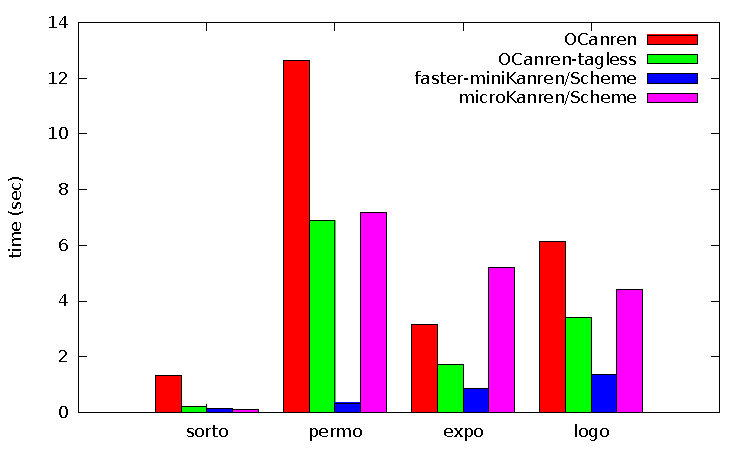
\includegraphics{graph1.pdf}
\caption{The First Set of Benchmarks}
\label{eval:first}
\end{figure}

\begin{figure}[h]
\centering
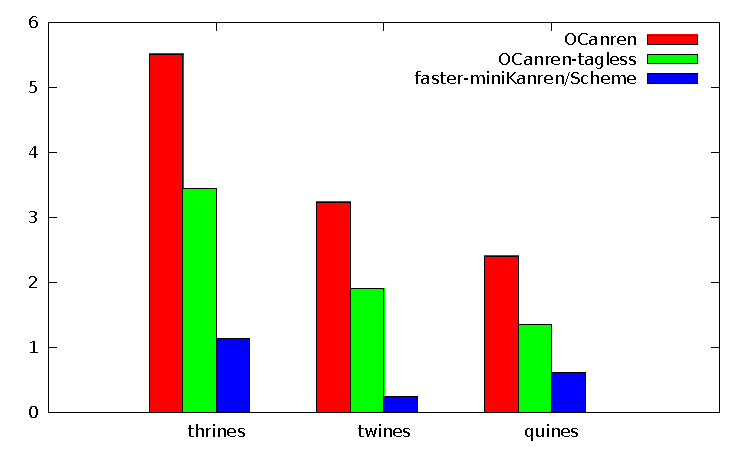
\includegraphics{graph2.pdf}
\caption{The Second Set of Benchmarks}
\label{eval:second}
\end{figure}

\section{Conclusion}

We presented a strongly-typed implementation of \miniKanren for OCaml. Our implementation
passes all tests written for \miniKanren (including those for disequality constraints);
in addition we implemented many interesting relational programs known from
the literature. We claim that our implementation can be used both as a convenient
relational DSL for OCaml and an experimental framework for future research in the area of
relational programming.

%We also want to express our gratitude to William Byrd, who infected us with relational programming,
%and for the extra time he sacrificed as both our tutor and friend.


\bibliographystyle{splncs04}
\bibliography{references}
\end{document}
